\documentclass[12pt]{article} % 

\usepackage[hyperfootnotes=false]{hyperref}
\usepackage[margin=1in]{geometry}                                              
\usepackage{amsmath,amsthm,amssymb}                                            
\usepackage{graphicx}                                                          
\graphicspath{{../data/}}
\usepackage{titlesec}                                                   
\usepackage{bm}
\usepackage{cprotect}
\usepackage{ bbold }
\usepackage{abstract}
\usepackage{biblatex}
\bibliography{bib.bib}
       
\usepackage{listings}
\lstset{basicstyle=\ttfamily,breaklines=true}

\titleformat{\subsection}[runin]
{\normalfont\large\bfseries}{\thesubsection}{1em}{}

\renewcommand{\bf}{\mathbf}
\renewcommand{\cal}{\mathcal}
\newcommand{\pd}[2]{\frac{\partial #1}{\partial #2}}
\newcommand{\pdn}[3]{\frac{\partial^{#3} #1}{\partial #2^{#3}}}
\newcommand{\pdop}[1]{\frac{\partial}{\partial #1}}
\newcommand{\nd}[2]{\frac{d #1}{d #2}}
\newcommand{\ndn}[3]{\frac{d^{#3} #1}{d #2^{#3}}}
\newcommand{\ndop}[1]{\frac{d}{d #1}}
\newcommand{\dt}{\frac{d}{dt}}
\newcommand{\grad}{\bm\nabla}
\newcommand{\cross}{\times}
\newcommand{\curl}{\grad\cross}
\newcommand{\imp}{\Longrightarrow\quad}
\newcommand{\abs}[1]{\left|#1\right|}
\newcommand{\half}{\frac{1}{2}}
\newcommand{\third}{\frac{1}{3}}
\renewcommand{\th}[1]{\frac{1}{#1}}
\renewcommand{\k}{4\pi\epsilon_0}
\newcommand{\eps}{\epsilon_0}
\newcommand{\intt}{\int_{t_1}^{t_2}}
\newcommand{\inti}{\int_{-\infty}^{+\infty}}
\newcommand{\ex}[1]{\left\langle #1 \right\rangle}
\renewcommand{\d}{\delta}
\newcommand{\e}{\text{e}}
\renewcommand{\l}{\ell}
\newcommand{\om}{\omega}
\newcommand{\h}{\hbar}
\newcommand{\ket}[1]{\left|#1\right\rangle}
\newcommand{\bra}[1]{\left\langle#1\right|}
\newcommand{\braket}[2]{\left\langle#1\middle|#2\right\rangle}
\newcommand{\brakett}[3]{\left\langle#1\middle|#2\middle|#3\right\rangle}
\newcommand{\comm}[2]{\left[#1,#2\right]}
\newcommand{\acom}[2]{\left\{#1,#2\right\}}
\newcommand{\nn}{\nonumber\\}

\DeclareMathOperator{\Tr}{Tr}

%\renewcommand{\thesection}{\arabic{section}}

\begin{document}

\title{\textbf{Majorana Fermions}}
\author{Charles Stahl}

\maketitle
%
%\section{Introduction} 
%
%To discuss Majorana fermions, it is helpful to discuss Dirac fermions, the first realization of relativistic fermions.
%
%\subsection{Dirac Equation}\footnote{How relevant is this? Should I cut some of it out?} \emph{}
%
%The Dirac equation can be derived by trying to mirror the nonrelativistic Shr\"odinger equation while obeying relativity. This derivation follows reference~\cite{gottfried03}. A problem with the nonrelativistic Shr\"odinger equation is that it does not treat time and space equally, in that it is first order in time and second order in space
%\begin{align}
%i\pdop{r}\psi(\bm r, t) &= \left[\frac{-1}{2m}\grad^2 +V(\bm r,t)\right]
%	\psi(\bm r, t). \label{eqn:shro}
%\end{align}
%Using the replacements
%\begin{align}
%\bm p \leftrightarrow \th{i}\grad, \quad E \leftrightarrow \th{i}\pdop{t}, 
%	\label{eqn:repl}
%\end{align}
%equation~\ref{eqn:shro} becomes $E = p^2/2m +V$, which is true in classical mechanics. In relativistic mechanics, the energy-momentum relationship becomes $E^2 = m^2 +p^2$, which reduces to the classical equation in the limit $p<<m$. Using the replacements from equation~\ref{eqn:repl}, this is
%\begin{align}
%\frac{\partial^2}{\partial t^2}\psi(\bm r,t)=\left(\grad^2-m^2\right)\psi
%	(\bm r,t),\label{eqn:klein}
%\end{align}
%the Klein Gordon equation. There are two problems with this equation as it is. It is second order in time, and does not admit of a probability interpretation.
%
%The form suggests we might want to find an operator that we could call 
%\begin{align}
%\sqrt{\grad^2-m^2}
%\end{align}
%using the Taylor series of $\sqrt{\cdot}$ which, when applied twice to $\psi$, would produce
%\begin{align}
%(\grad^2-m^2)\psi.
%\end{align}
%This attempt does not end up working because the square root includes terms of arbitrarily high order~\cite{sakurai11}.
%
%However, using the partial derivative on Minkowski space 
%\begin{align}
%\partial_\mu = (\partial_t,\grad),\quad\partial^\mu = \eta^{\mu\nu}\partial_
%	\nu = (\partial_t, -\grad),\label{eqn:partial}
%\end{align}
%we can rewrite equation~\ref{eqn:klein} as 
%\begin{align}
%\left(\partial_\mu\partial^\mu + m^2\right)\psi &= \left(\eta^{\mu\nu}\partial_
%	\mu\partial_\nu + m^2\right)\psi.
%\end{align}
%Evidently, we want a solution of the form
%\begin{align}
%(i\gamma^\mu\partial_\mu - m)\psi = 0,
%\end{align}
%so that, by operating with the complex conjugate,
%\begin{align}
%(-i\gamma^\mu\partial_\mu - m)(i\gamma^\nu\partial_\nu - m)\psi =(\gamma^\mu
%	\gamma^\nu\partial_\mu\partial_\nu + m^2) = 0. \footnote{Is this satisfying?}
%\end{align}
%Note that partial derivatives with different indices commute
%
%Since the partial derivative commutes, $\partial_\mu\partial_\nu$ is symmetric, so we can require that the $\gamma$ term above is symmetric as well.
%\begin{align}
%\gamma^\mu\gamma^\nu = \half\left(\gamma^\mu\gamma^\nu + \gamma^\nu\gamma^\mu
%	\right) = \{\gamma^\mu,\gamma^\nu\} = \eta^{\mu\nu}
%\end{align}
%This antisymmetry requirement is central to the Dirac equation.\footnote{This derivation is a mix of Gottfried and Sakurai. I think Gottfried has a better derivation in a different place, but I haven't been able to understand it. I plan to read it again this weekend and have a better writeup for this section.}
%
%\subsection{Antiparticles}
%
%\subsection{Fermion Second Quantization}\emph{}
%
%Before fermionic second quantization it is convenient to consider the bosonic case. Bosonic fields such as the electromagnetic field can be decomposed into modes $\bm p$ with raising and lowering operators $a^\dagger_{\bm{p}}$ and $a_{\bm{p}}$. Since the number of particles is not fixed, the Hilbert space spans subspaces of different $N'$. This is called the Fock Space $\mathfrak{F}$,
%\begin{align}
%\mathfrak{F} = \mathfrak{H}_0 \oplus \mathfrak{H}_1 \oplus \mathfrak{H}_2 
%	\oplus \cdots
%\end{align}
%where $\mathfrak{H}_N'$ is the subspace with $N'$ particles. 
%
%The vacuum state is written as $\ket{0}$. A state with one particle in mode $\bm p_1$ is $a^\dagger_{\bm p_1}\ket{0} = \ket{\bm p_1}$. Since bosonic states must be symmetric, the state $\ket{\bm p_1\bm p_2} = a^\dag_{\bm p_1} a^\dag_{\bm p_2}\ket{0}$ must equal to $\ket{\bm p_2\bm p_1} = a^\dag_{\bm p_2} a^\dag_{\bm p_1}\ket{0}$. From this we derive the boson commutation relations
%\begin{align}
%[a^\dag_{\bm p}, a^\dag_{\bm p'}] = [a_{\bm p}, a_{\bm p'}]=0.
%\end{align}
%The only nonzero commutation is 
%\begin{align}
%[a_{\bm p},a^\dag_{\bm p'}] = \d_{\bm{p,p}'}
%\end{align}
%
%Since these operators create and annihilate particles, they can define a number operator $N_{\bm p} = a^\dagger_{\bm p}a_{\bm p}$ with eigenvalues $N'_{\bm p}$ which count the particles in mode $\bm p$. The total number of particles is $N' = \sum_{\bm p}N'_{\bm p}$.\footnote{Is it correct to introduce the number operator as a result of the commutation relations (are the commutation relations the fundamental part)?}
%
%Second quantization for fermions must be fundamentally different. Only one fermion can exist in any mode. A fermionic state is then a series of bits; 1 if a particle exists in the corresponding mode and 0 if the mode is unoccupied. Furthermore, the state must be antisymmetric. Therefore the state
%\begin{align}
%\ket{\alpha_{\nu_1}\alpha_{\nu_2}\alpha_{\nu_3}\cdots\alpha_{\nu_N}}
%\end{align}
%is shorthand for 
%\begin{align}
%\ket{\alpha_{\nu_1}\alpha_{\nu_2}\alpha_{\nu_3}\cdots\alpha_{\nu_N}}_A = 
%	\epsilon^{ijk\cdots n}\ket{\alpha_{\nu_i}\alpha_{\nu_j}\alpha_{\nu_k}\cdots
%	\alpha_{\nu_n}}.
%\end{align}
%Here, the $\nu_i$ are some quantum numbers (not necessarily momentum modes). $\epsilon$ is the totally antisymmetric tensor with $N$ indices, where $n$ is the $N$th index.
%
%%  Anticommutation relations??
%
%This means that, when defining operators in terms of $\psi$ operators, it is convenient to define them with the operators in canonical order, for example
%\begin{align}
%\cal A = \sum_{i<j<k}A^{ijk}a_ia_ja_k.
%\end{align}
%If $A$ is defined to be antisymmetric, 
%\begin{align}
%\cal A = \th{N!}\sum_{ijk}A^{ijk}a_ia_ja_k,
%\end{align}
%where $N$ is the number of operators. 



\section{Supersymmetry in Oscillators}

\subsection{Bosonic and Fermionic Oscillators} \emph{}

One starting point for discussing supersymmetry is through the formalism of harmonic oscillators.\footnote{I spent a lot of time debating how to start talking about creation and annihilation. How should I?} First consider a single harmonic oscillator 
\begin{align}
H = p^2 +\om^2 x^2,\quad \comm{x}{p} = \frac{i}{2}. \label{eqn:harmosc}
\end{align}
The raising and lowering operators 
\begin{align}
a = \sqrt{\om}x+\frac{i}{\sqrt{\om}}p,\quad a^\dag = \sqrt{\om}x+\frac{i}{
	\sqrt{\om}}p,\quad \comm{a}{a^\dag } = 1.
\end{align}
The Hamiltonian can then be written as 
\begin{align}
H = \om a^\dag a + \th{2} \equiv \om N + \th{2}.
\end{align}
After introducing a ground state $\ket{0}$ such that $a\ket{0} = 0$, the number operator $N$ counts the number of times the raising operator has been applied to a state. This shows that the raising and lowering operators add and remove energy from the system, respectively. 

The Hamiltonian for electromagnetism can be written as
\begin{align}
H = \sum_p \left(P_p^2 + \om_p^2x_p^2\right)
\end{align}
with the proper choice of $x$ and $P$. Given a collection of modes $p$ with frequencies $\om_p$ and creation and annihilation operators $a_p^\dag$ and $a_p$, the commutation relations become 
\begin{align}
[a_p, a_{p'}] = 0,\quad [a^\dag_p, a^\dag_{p'}]=0, \quad[a_p,a^\dag_{p'}] = 
	\delta_{p,p'},
\end{align}
and the Hamiltonian becomes
\begin{align}
H = \sum_p\left(\om_pN_p+\th{2}\right),
\end{align}
meaning that acting with $a_p^\dag$ adds $\om_p$ to the energy of the state.

The interpretation is that each raising operator $a_p$ adds a photon with energy $\om_p$, for which it is called the creation operator. Likewise, $a_p^\dag$ is called the annihilation operator. Then, $N_p$ counts the number of photons with energy $\om$. Since particle number is not conserved, the state space is now a  Fock Space $\mathfrak{F}$,
\begin{align}
\mathfrak{F} = \mathfrak{H}_0 \oplus \mathfrak{H}_1 \oplus \mathfrak{H}_2 
\oplus \cdots
\end{align}
where $\mathfrak{H}_N$ is the subspace with $N$ particles. Actually, it a product of Fock spaces, one for each value of $p$.\footnote{Is this true?}

States with definite values of $N_p$ are stationary states, and can be specified by the number of particles in each mode $\{n_p\}$. Since the space is a product over $p$ of spaces for each mode, these states can be written as
\begin{align}
\ket{\{n_p\}} = \prod_pa_p^\dag\ket{0}.
\end{align}
Since operators for different modes commute, we have
\begin{align}
\ket{p_1p_2} = a^\dag_{p_1}a^\dag_{p_2}\ket{0} = a^\dag_{p_2} a^\dag_{p_1} \ket{0} = \ket{p_1p_2},
\end{align}
which is to say that the states are symmetric.

Fermionic operators obey the anticommutation relations
\begin{align}
\{b_p, b_{p'}\} = 0,\quad \{b^\dag_p, b^\dag_{p'}\} = 0,\quad \{b_p, b^\dag_{p'}\} = \delta_{p,p'}.
\end{align}
The analysis of the Fock space matches that for bosonic operators, except the states are are antisymmetric because
\begin{align}
\ket{p_1p_2} = b^\dag_{p_1}...
\end{align}

Unlike in the case of bosons, there cannot be an arbitrary number of fermions in a mode, but rather at most one. This can be seen by trying to raise a non-empty state: $b_p^\dag b^\dag_p\ket{0} = 0$. The operators maintain their interpretation as creation and annihilation operators, though.

\subsection{Majorana Fermions} \emph{}

The algebra of Majorana fermions is closely related to that of normal (Dirac) fermions, with the difference being a lack of annihilation operator
\begin{align}
\{\psi_p,\psi_{p'}\} = \delta_{p,p'}.
\end{align}
This leads to antisymmetric states, like the Dirac Fermion, but allows for no antiparticles.\footnote{I still don't understand this. How do I not understand this?}

\subsection{Supersymmetry} \emph{}



\section{SYK Model}

All sums of operators are defined such that the operators are in canonical order.

\subsection{Definition} \emph{}

The SYK model is defined as having a Hamiltonian
\begin{align}
H = \sum_{ijk\l}J_{ijk\l}\psi^i\psi^j\psi^k\psi^\l,
\end{align}
where $J_{ijk\l}$ are drawn from a normal distribution. The operators obey the anticommutation relations
\begin{align}
\{\psi^i,\psi^j\} = \delta^{ij}.
\end{align}

\subsection{Initial Calculations}

\subsection{Large $N$ Limit}

\subsection{Supersymmetry}\emph{}

The discussion of the supersymmetric models comes from reference~\cite{fu16}. In the supersymmetric generalization, the Hamiltonian is written in terms of the supercharge
\begin{align}
Q = i\sum_{i<j<k}C_{ijk}\psi^i\psi^j\psi^k,
\end{align}
where $C_{ijk}$ are now drawn from a Gaussian with mean 0 and variance $2J/N^2$. Because the $\psi$ operators are antisymmetric, the other components of $C$ may be chosen so that $C$ is also antisymmetric. In this case 
\begin{align}
Q = \frac{i}{6}\sum_{ijk}C_{ijk}\psi^i\psi^j\psi^k,
\end{align}
with the indices no longer necessarily ordered.

The Hamiltonian is defined as
\begin{align}
H &= Q^2 = - \sum_{i<j<k}C_{ijk}\psi^i\psi^j\psi^k\sum_{\l<m<n}C_{\l mn}\psi^\l
	\psi^m\psi^n.
\end{align}
For those terms where $(i,j,k) = (\l,m,n)$, the sum becomes
\begin{align}
\sum_{i<j<k}C_{ijk}^2\psi^i\psi^j\psi^k\psi^i\psi^j\psi^k = \th{8} \sum_{i<j<k}
	C_{ijk}^2 
\end{align}
Eventually\footnote{I'm not able to derive this. What am I missing?} the Hamiltonian becomes
\begin{align}
H = E_0 + \sum_{i<j<k<\l}J_{ijk\l}\psi^i\psi^j\psi^kk\psi^\l, \label{eqn:N1def}
\end{align}
where
\begin{align}
E_0 = \sum_{i<j<k} C_{ijk}^2\;,\qquad J_{ijk\l} = -\th{8}\sum_{a} C_{a[ij}
	C_{kl]a}.
\end{align}
This shows that $E_0$ is positive, with expectation (over the values of $C_{ijk}$)
\begin{align}
\ex{E_0} &= \sum_{i<j<k}\ex{C^2_{ijk}}\nn
&= \th{6}N(N-1)(N-2)\frac{2J}{N^2}.
\end{align}
In the large $N$ limit this becomes $E_0 = NJ/3$.\footnote{This contradicts the Fu paper's assertion that $E_0\to 0$ for large $N$. What am I missing?}

\subsection{$\cal{N}=2$ Supersymmetry, Ground States}\emph{}

In $\cal N=2$ supersymmetry, two supercharges are necessary. To create these, define a new set of fermions that consists of $\psi^i$ and their conjugates $\bar{\psi_i}$. These obey the relations 
\begin{align}
\{\psi^i,\psi^j\} = 0, \quad \{\bar{\psi_i},\bar{\psi_j}\} = 0, \quad
	\{\psi^i,\bar{\psi_j}\} = \delta_j^i. \label{eqn:N2_ant}
\end{align}
The supercharges are 
\begin{align}
Q &= i\sum_{i<j<k}C_{ijk}\psi^i\psi^j\psi^k,\quad
\bar{Q} = i\sum_{i<j<k}\bar C^{ijk}\bar{\psi_i}\bar{\psi_j}\bar{\psi_k},
	\label{eqn:N2charge}
\end{align}
where the $C_{ijk}$ are complex numbers drawn from a 0-centered Gaussian such that
\begin{align}
\ex{C_{ijk}\bar C^{ijk}} = \frac{2J}{N^2}.
\end{align} 
The Hamiltonian is defined as 
\begin{align}
H &= \{Q, \bar Q\} = \cdots\nn
&= E_0 + \sum_{ijk\l}J_{ij}^{k\l}\psi^i\psi^j\bar{\psi_k}\bar{\psi_\l}.
\end{align}
Like in the $\cal N=1$ case, the components of $J$ are no longer independent. 

The operators $Q^2$ and $\bar Q^2$ are both 0. That implies that both $Q$ and $\bar Q$ are conserved, as for example
\begin{align}
[H,Q] = Q\bar QQ + \bar QQQ - QQ\bar Q + Q\bar QQ = 0.
\end{align}
This also means they preserve energy. This last fact suggests a convenient way of counting ground states.

Consider a stationary state $\ket{\phi_E}$ with energy $E$. Consider also the states $\ket{q_E} = Q\ket{\phi_E}$ and $\ket{\bar q_E}= \bar Q \ket{\phi_E}$. These states will have the same energy eigenvalue $E$, if they exist. If $Q$ and $\bar Q$ annihilate $\ket{\psi_E}$, then $E=0$. If $\bar Q$ annihilates $\ket{\phi_E}$ but $Q$ does not, then 
\begin{align}
H\ket{\phi_E} = (Q\bar{Q} + \bar QQ)\ket{\phi_E} = \bar QQ\ket{\phi_E} = E\ket{\phi_E}
\end{align}
and the state $\ket{f_E} = \bar QQ\ket{\phi_E}$ is just $\ket{\phi_E}$, $E>0$. The same analysis applies if $Q$ annihilates but $\bar Q$ does not.

If both $\ket{q_E}$ and $\ket{\bar q_E}$ exist and $E>0$, then
\begin{align}
H\ket{\phi_E} = E\ket{\phi_E} = (Q\bar Q + \bar QQ)\ket{\phi_E} = \ket{f_E} + 
	\ket{f'_E},
\end{align}
meaning 
\begin{align}
\ket{f_E} = \alpha\ket{\phi_E} + \beta\ket{\xi_E},\qquad \ket{f'_E} = 
	(1-\alpha)\ket{\phi_E} - \beta\ket{\xi_E}.
\end{align}
$\ket{\xi_E}$ must exist for $\ket{q_E}$ and $\ket{\bar q_e}$ to be distinct.

The previous analysis divides the space into tuplets of energy eigenstates with at most 4 members. See figure~\ref{fig:tuplets}. All tuplets contain an even number of states, except for some of the ground state tuplets. All even tuplets contain an equal number of fermionic and bosonic states.
\begin{figure}
	\centering 
	\caption{\textbf{Illustration of the possible configuration of energy eigenstate tuplets.} This illustration does not exist yet.}
	\label{fig:tuplets}
\end{figure}

This provides the opportunity to count ground states using the Fermi number
\begin{align}
F = \sum_i\bar{\psi_i}\psi^i,
\end{align}
which is even for bosonic states and odd for fermionic states. The operator 
\begin{align}
\Tr\left((-1)^F\right) \label{eqn:N2witten}
\end{align}
has contributions only from the ground states, so the number of ground states will be equal to or greater than $|F|$. Similarly, the Witten index
\begin{align}
W = \Tr\left((-1)^F\e^{\beta H}\right)
\end{align}
is independent of temperature because $H$ is zero in the ground states. The Witten index is also independent of coupling, so it can be computed with $J=0$. Then the Witten index is just equation~\ref{eqn:N2witten}.

Define the unitary operator 
\begin{align}
R^p = \e^{\frac{2\pi ipF}{3}},\quad R^3 = \mathbb{1}.
\end{align}
$R$ commutes with $Q$ so that
\begin{align}
\Tr\left((-1)^FR^p\right)
\end{align}
also only has contributions from the ground state. Eventually,\footnote{How?} it can be shown that
\begin{align}
W = \left(1-\e^{\frac{2\pi ip}{3}}\right)^N = \e^{\frac{iN\pi}{den}}
\end{align}
and the dimension of ground states is 
\begin{align}
\abs{W} = \sqrt{3}^N,
\end{align}
while the dimension of the whole space is 
\begin{align}
2^N.
\end{align}

\section{Numerical Results}

\subsection{Building Matrices}\emph{}

The simplest way to compute large-N functions on a computer is to use a matrix representation for the group. This can be done by viewing the $\bar \psi$ and $\psi$ operators as raising and lowering operators, respectively. Consider the case of $N$ fermions. Write the state as an $N$-dimensional binary vector \footnote{I want to include this because I spent a lot of time on it. Is that ok?}
\begin{align}
\ket{m} = \ket{m_1m_2\dots m_i\dots m_{N-1}m_N}, \quad\sum_nm_n2^{n-1} =
	m.\label{eqn:2Nstate}
\end{align}
The vacuum state is $\ket{0}$. A populated state can be written as
\begin{align}
\ket{110\dots 0} = \bar\psi_1\bar{\psi_2}\ket{0} =-\bar\psi_2\bar\psi_1\ket{0},
\end{align}
which enforces the canonical ordering through anticommutation relations. 

The matrix representations of $\psi^i, \bar \psi_i$ are then calculated component-wise using an $2^N$ by $2^N$ matrix.
\begin{align}
\bar\psi_i &= \sum_{a,b}\ket{a}\bar\psi_{i,ab}\bra{b}\nn
\bar\psi_{i,ab} &= \brakett{a}{\bar\psi_i}{b}.\label{eqn:comps}
\end{align}
These components may be calculated effectively using the pseudocode in figure~\ref{code:psibar}.\footnote{Should I explain the code more?}

\begin{figure}
	\begin{lstlisting}[language=python][gobble=2]
    def psi_bar(N,i):
      psi_bar = np.zeros((2^N,2^N))
      for (n,m) in psi_bar:
        if (m-n == 2^j) and (n & 2^j == 0): 
          psi[m,n] = (-1)^Fermi(n,j),
    return psi_bar
		\end{lstlisting}
	\cprotect\caption{\textbf{Code for generating $\bar \psi$ matrices,} where \verb|^| represents exponentiation, \verb|&| represents bitwise and \verb|Fermi(n,j)|, the reduced Fermi number, is the number of nonzero components in \verb|n| before the \verb|j|'th component. This handles anticommutation requirements. A similar structure can be used for building the $\psi$ matrices.}
	\label{code:psibar}
\end{figure}

It is also possible to create the matrices recursively. The base case is $N=1$, for which the matrices are the raising and lowering matrices,
\begin{align}
\bar\psi_{0,(1)} = \begin{bmatrix} 0&0\\1&0 \end{bmatrix}, \qquad
    \psi^0_{(1)} = \begin{bmatrix} 0&1\\0&0 \end{bmatrix}. \label{eqn:base}
\end{align}
Then, to increase the dimension take the tensor product with the $2\times 2$ identity matrix $I$,
\begin{align}
\bar\psi_{i,(N)} = I\otimes\bar\psi_{i,(N-1)},\quad \psi^i_{(N)} = I\otimes 
	\psi^i_{(N-1)}.
\end{align}
This formula of course does not work when $i=N$. In this case the solution is still to use recursion, with the formula
\begin{align}
\bar\psi_{i,(N)} = \bar\psi_{i,(N-1)}\otimes\sigma_3,
\end{align}
with equation~\ref{eqn:base} again supplying the base case.

Although there are various representations of the group, the previous two constructions lead to the same representation. 

\subsection{Ground States} \emph{}

Counting ground states was implemented by counting the zero eigenvalues of a randomly-generated Hamiltonian. The number of ground states stayed above the bound, although the bound was not tight in some places. See figure~\ref{fig:gserr} for the ground states above the bound.\footnote{Would this graph be better as actual/predicted?}

\begin{figure}
	\centering
	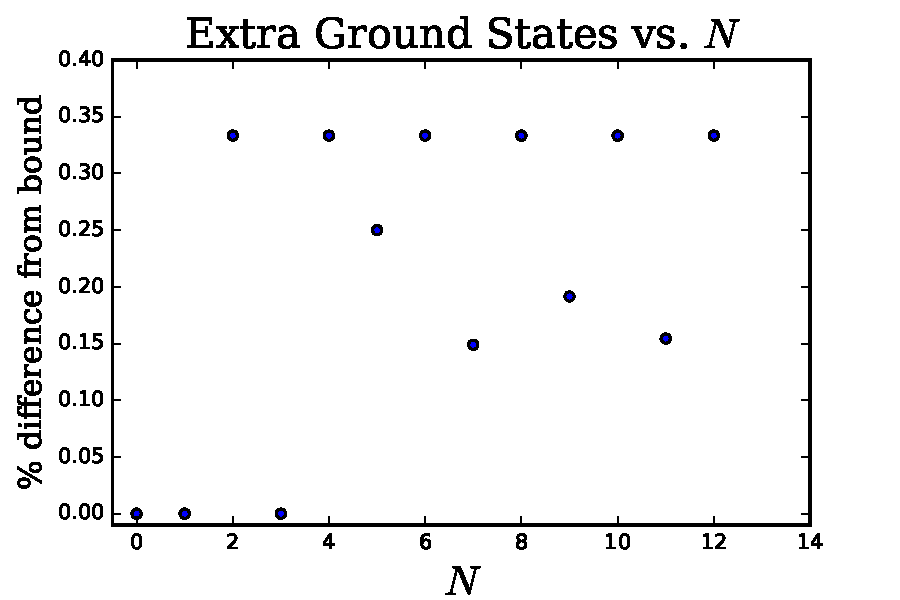
\includegraphics[width=.5\textwidth]{gserr}
	\caption{\textbf{Looseness of bound on number of ground states.} 0 represents the bound being tight while 1 would mean twice as many ground states as the bound. Since the number of ground states is an integer, these values were calculated as $\text{ceil}(\sqrt{3}^N)$.}
	\label{fig:gserr}
\end{figure}

It is particularly interesting to note that the number of ground states is particularly high for even $N$. Even with randomly generated Hamiltonians, the relative number of ground states above the bound stays relatively constant near 0.33. 

\subsection{Ground State Entanglement Entropy}

Once the number of ground states were calculated for a single Hamiltonian, the entropy of a subsystem\footnote{Terminology?} of the ground state could be calculated from the reduced density matrix of the subsystem. Starting with a ground state $\ket{\phi}$, the density matrix $\rho = \ket{\phi}\bra{\phi}$ can be calculated. The entropy $S = \Tr\rho\log\rho$ can be calculated as 
\begin{align}
S = \sum \lambda\log\lambda,
\end{align}
where $\lambda$ are the eigenvalues. 

As predicted, the entropy rises and drops linearly as more particles are traces over. Since the entropy does not depend on the coupling, a single computation of the entropy should be sufficient.\footnote{Right?} However, due to small numerical errors, it is helpful to perform multiple calculations and average the entropies. 



\printbibliography

\end{document}
